\section{Results}
We analyzed short-term effects of \gls{RP} on accelerations, position, and Keplerian orbital elements. While position and orbital elements are ultimately relevant for precise orbit determination, examining the accelerations in different scenarios and along the orbit can explain why position and orbital elements changed. Additionally, the accelerations highlight differences between models of varying complexity.

To compare accelerations over one or multiple orbits, we used the \gls{RMSE}, which is defined as
\begin{align}
    \text{RMSE}(x, y) = \sqrt{\frac{1}{n}\sum_{i=1}^{n}\left(x_i - y_i\right)^2}.
\end{align}
The \gls{RMSE} describes the difference between two scalar timeseries $x_i, y_i$ and gives more weight to large deviations. These scalar timeseries can be the magnitude of accelerations or individual components. The \gls{rRMSE} is defined as
\begin{align}
    \text{rRMSE}(x, y) = \sqrt{\frac{\sum_{i=1}^{n}\left(x_i - y_i\right)^2}{\sum_{i=1}^{n} y_i^2}}
\end{align}
and is useful to compare differences across orders of magnitude.

While the simulation evaluates accelerations in a global frame, the effect of accelerations on the orbit is best analyzed in a spacecraft-fixed coordinate system that is aligned with the orbital track. The RSW coordinate system is one such system, defined by the unit vectors~\cite{Vallado2013}
\begin{align}
    \vb R = \frac{\vb r}{\norm{\vb r}}, \quad
    \vb W = \frac{\vb r \times \vb v}{\norm{\vb r \times \vb v}},
    \quad \textrm{and} \quad \vb S = \vb W \times \vb R.
\end{align}
The radial component $\vb R$ is aligned with the planetocentric position vector $\vb r$. The cross-track component $\vb W$ is aligned with the angular momentum vector, or orbit plane normal, involving the linear velocity $\vb v$. The along-track component $\vb S$ completes the right-handed coordinate system. Note that $\vb S$ is generally not aligned with the velocity vector, only for circular orbits.





\subsection{Instantaneous reradiation}
\label{subsec:inst-rerad}

First, we investigated the effect of instantaneous reradiation for the paneled target model. This increases the acceleration proportional to each panel's $C_a$, normal to the panel (cf. \cref{eq:brdf-reaction-specular-diffuse-instrerad}).

\begin{figure}[t]
    \centering
    \begin{subfigure}[c]{\linewidth}
        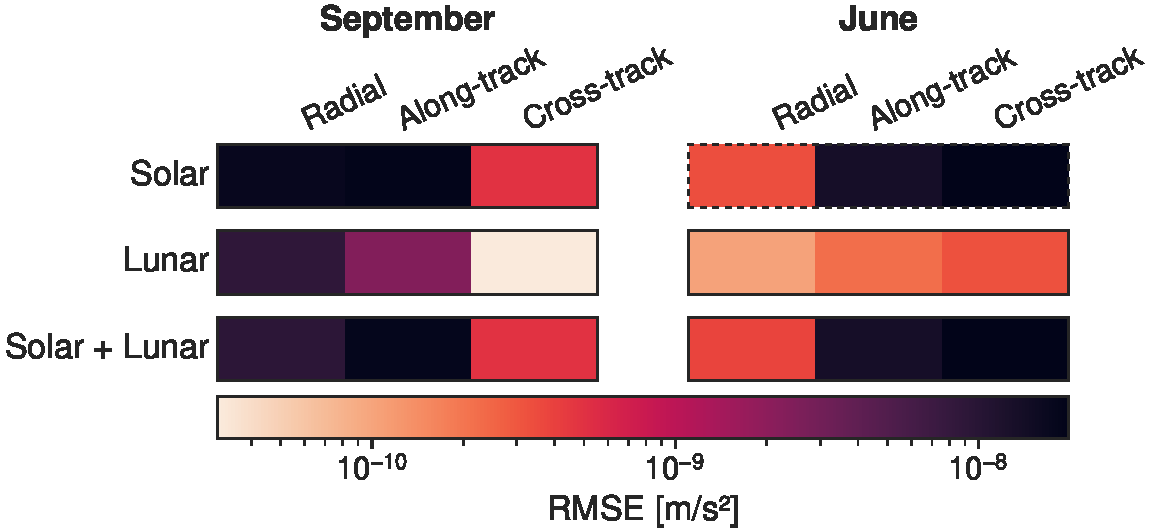
\includegraphics[width=\textwidth]{figures/plots/acc_reradiation_rms.pdf}
        \subcaption{Absolute}
     \end{subfigure}

     \bigskip

     \begin{subfigure}[c]{\linewidth}
        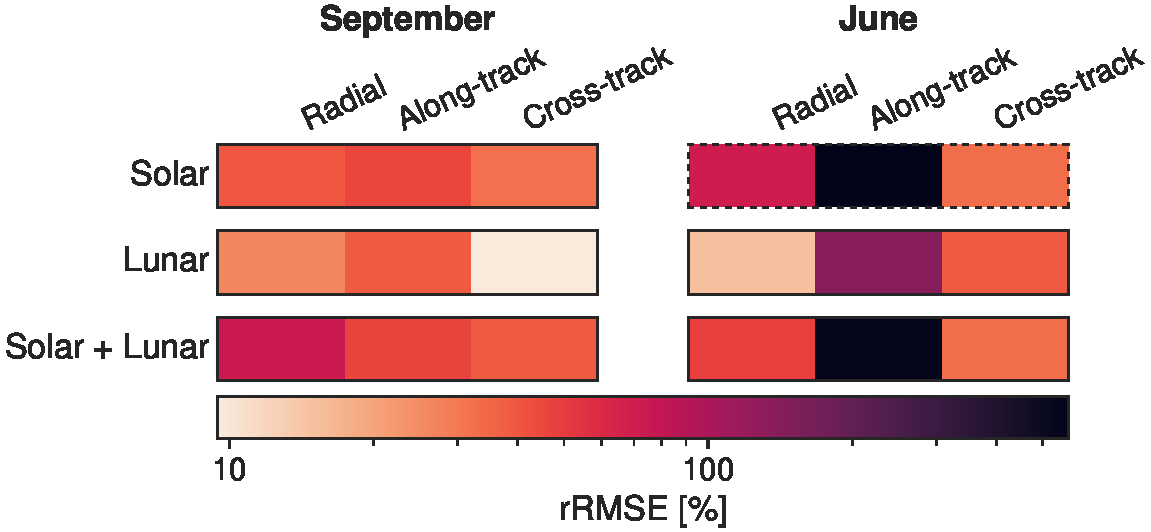
\includegraphics[width=\textwidth]{figures/plots/acc_reradiation_rrms.pdf}
        \subcaption{Relative}
     \end{subfigure}
    \caption{RMS differences of \gls{RP} accelerations over one orbit with and without instantaneous reradiation. The dashed boxes correspond to \cref{fig:acc-reradiation}.}
    \label{fig:acc-reradiation-rms}
\end{figure}

\begin{figure}[t]
    \centering
    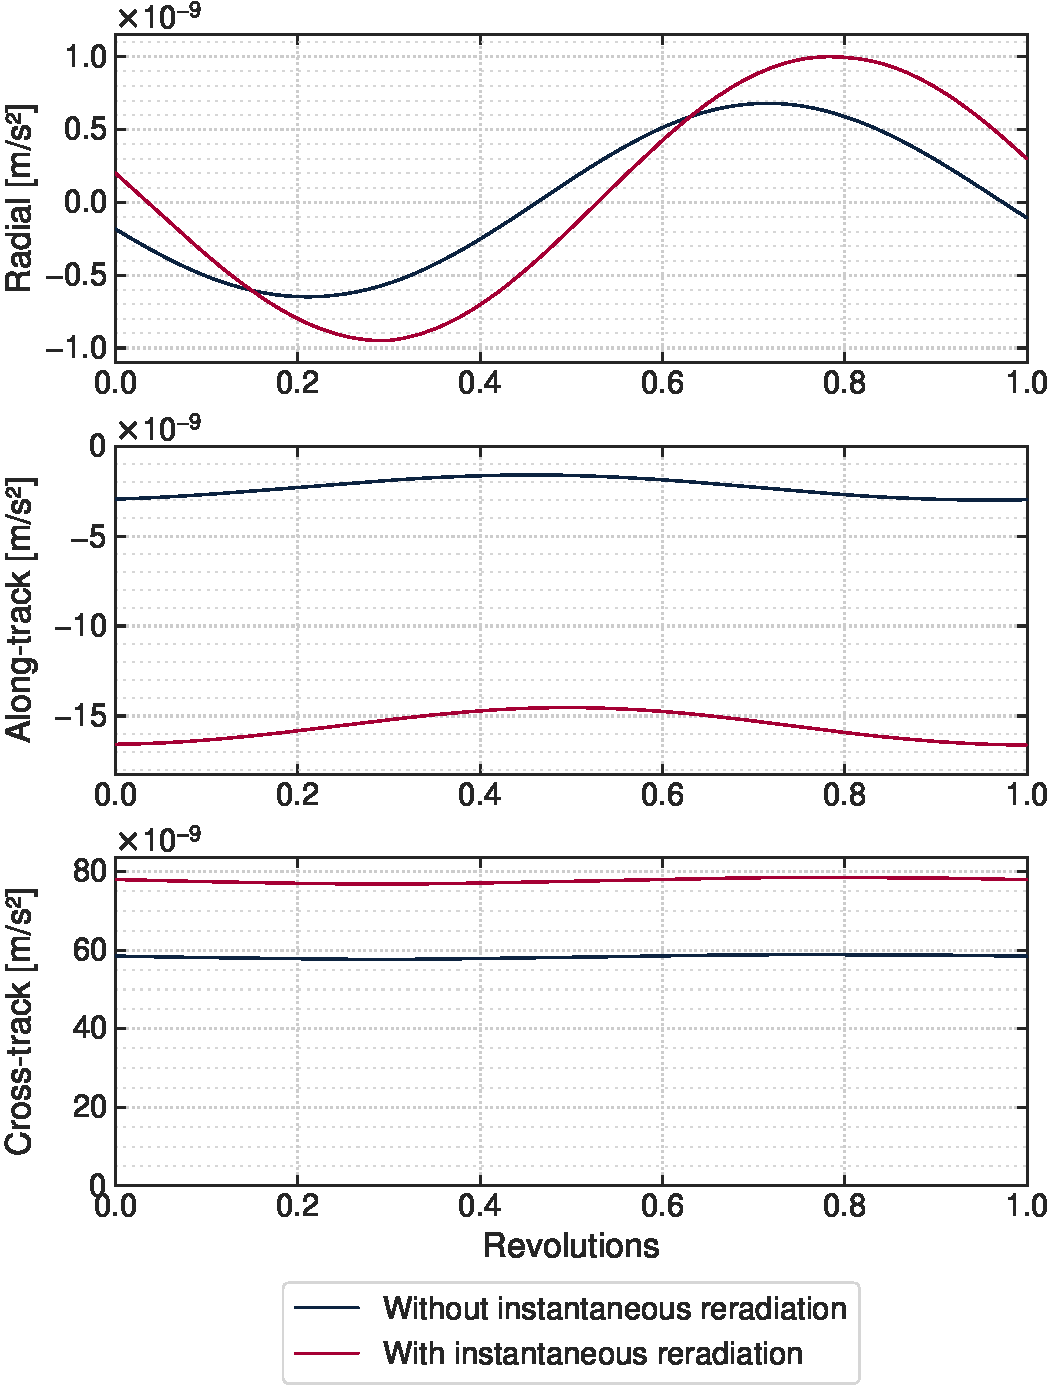
\includegraphics[width=\linewidth]{figures/plots/acc_reradiation_sun_jun.pdf}
    \caption{Accelerations due to solar radiation without and with instantaneous reradiation over one orbit for June arc. There is a phase shift in the radial component and the along-track component increased by \qty{570}{\percent} \gls{RMSE}. Lunar contributions and the September arc are not sifnigicantly affected in shape.}
    \label{fig:acc-reradiation}
\end{figure}

\Cref{fig:acc-reradiation} shows the absolute and relative differences between accelerations without and with instantaneous reradiation. In absolute terms, the radial and along-track components are impacted most for the September arc, while the along-track and cross-track components experience the largest increase for the June arc (for both arcs, up to about \qty{1.9e-8}{\acc} \gls{RMSE}). The relative differences are more uniform (around \qty{40}{\percent} \gls{rRMSE}), but the along-track components of lunar and solar radiation in the June arc increase by \qty{140}{\percent} and \qty{570}{\percent} \gls{rRMSE}, respectively. In most cases, only the magnitude of accelerations changes but not their pattern.

\Cref{fig:acc-reradiation} shows the solar radiation of the June arc, the only of our simulations for which the pattern changed significantly. The phase of the radial acceleration is shifted by about \qty{10}{\percent} of the orbital period, which is not the case for the other two components or the acceleration due to lunar radiation. This arc also had the largest relative change in along-track acceleration as described above (highlighted in \cref{fig:acc-reradiation-rms}). This change is clearly visible as a constant offset of about \qty{13e-9}{\acc}. 

The large changes seen in some cases are mostly due to the +SA panel, which is highly absorptive ($C_a = 0.90$) and large ($A = \qty{11.00}{\m\squared}$). For the June arc, the solar array is angled at \qty{45}{\degree} with equal components in the cross-track and along-track directions The Sun is on the same side as the solar array in the cross-track direction. Without instantaneous reradiation, no panel has a significant contribution to the along-track acceleration, so it is quite small at around \qty{2e-9}{\acc}. With instantaneous reradiation, each panel, and especially the solar array, exerts an acceleration parallel to its normal, which leads to the along-track increase witnessed for the June arc.

We applied instantaneous reradiation for all of the following simulation since no reradiation due to spacecraft panels is physically unrealistic and the differences in magnitude are significant when instantaneous reradiation is added. More sophisticated thermal models involving conduction and internal heat production would likely give more accurate results.




% \subsection{Simulation setups}

% Solar with/without
% Lunar with/without
% Albedo none/constant/dlam
% Thermal none/angle-based
% LRO cannonball/paneled
% with/without isntantaneous reradiation
% Beta angle/arc

% 46 simulations





\subsection{Accelerations}
The most direct effect of \gls{RP} is visible in the accelerations. Therefore, we compare the \gls{RP} accelerations
\begin{itemize}
    \item for the September and June arcs,
    \item due to solar and lunar (albedo + thermal) radiation,
    \item for constant and \gls{DLAM1} albedo distributions,
    \item for cannonball and paneled targets.
\end{itemize}
In total, we ran 46 simulations. All accelerations are given in \qty{e-9}{\acc}. Regarding cannonball and paneled target models, note that their comparative magnitudes are less important since the cannonball parameters have large uncertainties. Instead, we compared their behavior and how it relates to model assumptions (e.g., symmetry for the cannonball, tracking for the paneled target).


\subsubsection{Solar and lunar radiation}
Both solar and lunar radiation are significant but their accelerations may amplify or cancel each other. To compare them, we used a constant albedo model in addition to the thermal model. The accelerations over one orbit are shown in \cref{fig:acc-solarvslunar}. Note that secular variations in orbit geometry can change the magnitude of acceleration components even within one 2.5 day arc but are not shown here.

\begin{figure*}[t]
    \centering
    \begin{subfigure}[c]{\textwidth}
        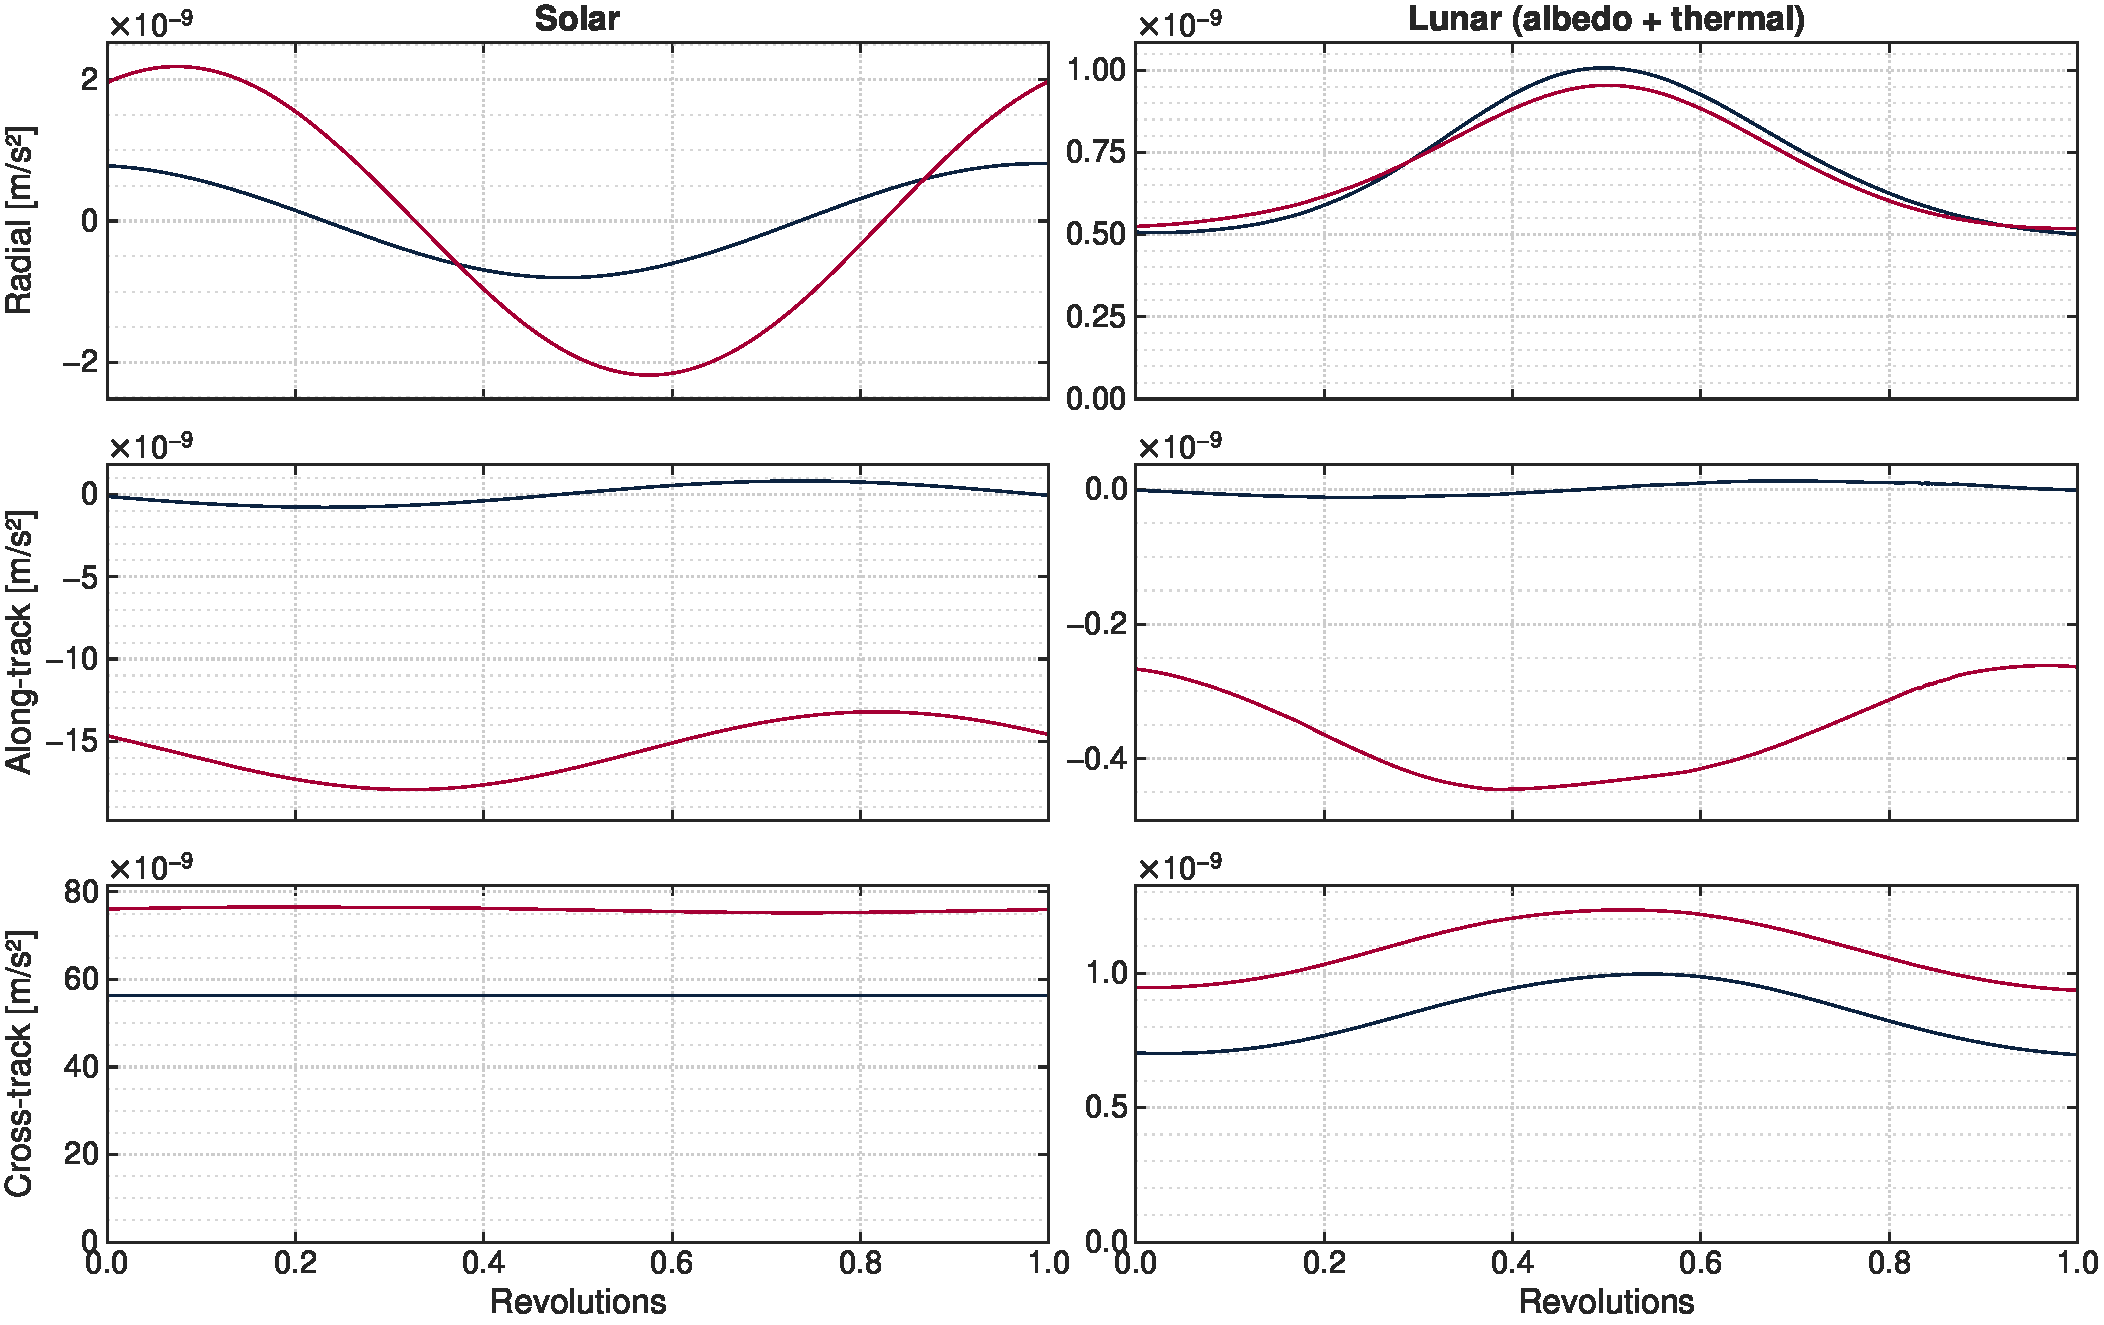
\includegraphics[width=\textwidth]{figures/plots/acc_solarvslunar_jun.pdf}
        \subcaption{June}
        \label{fig:acc-solarvslunar-jun}
     \end{subfigure}

     \bigskip

     \begin{subfigure}[c]{\textwidth}
        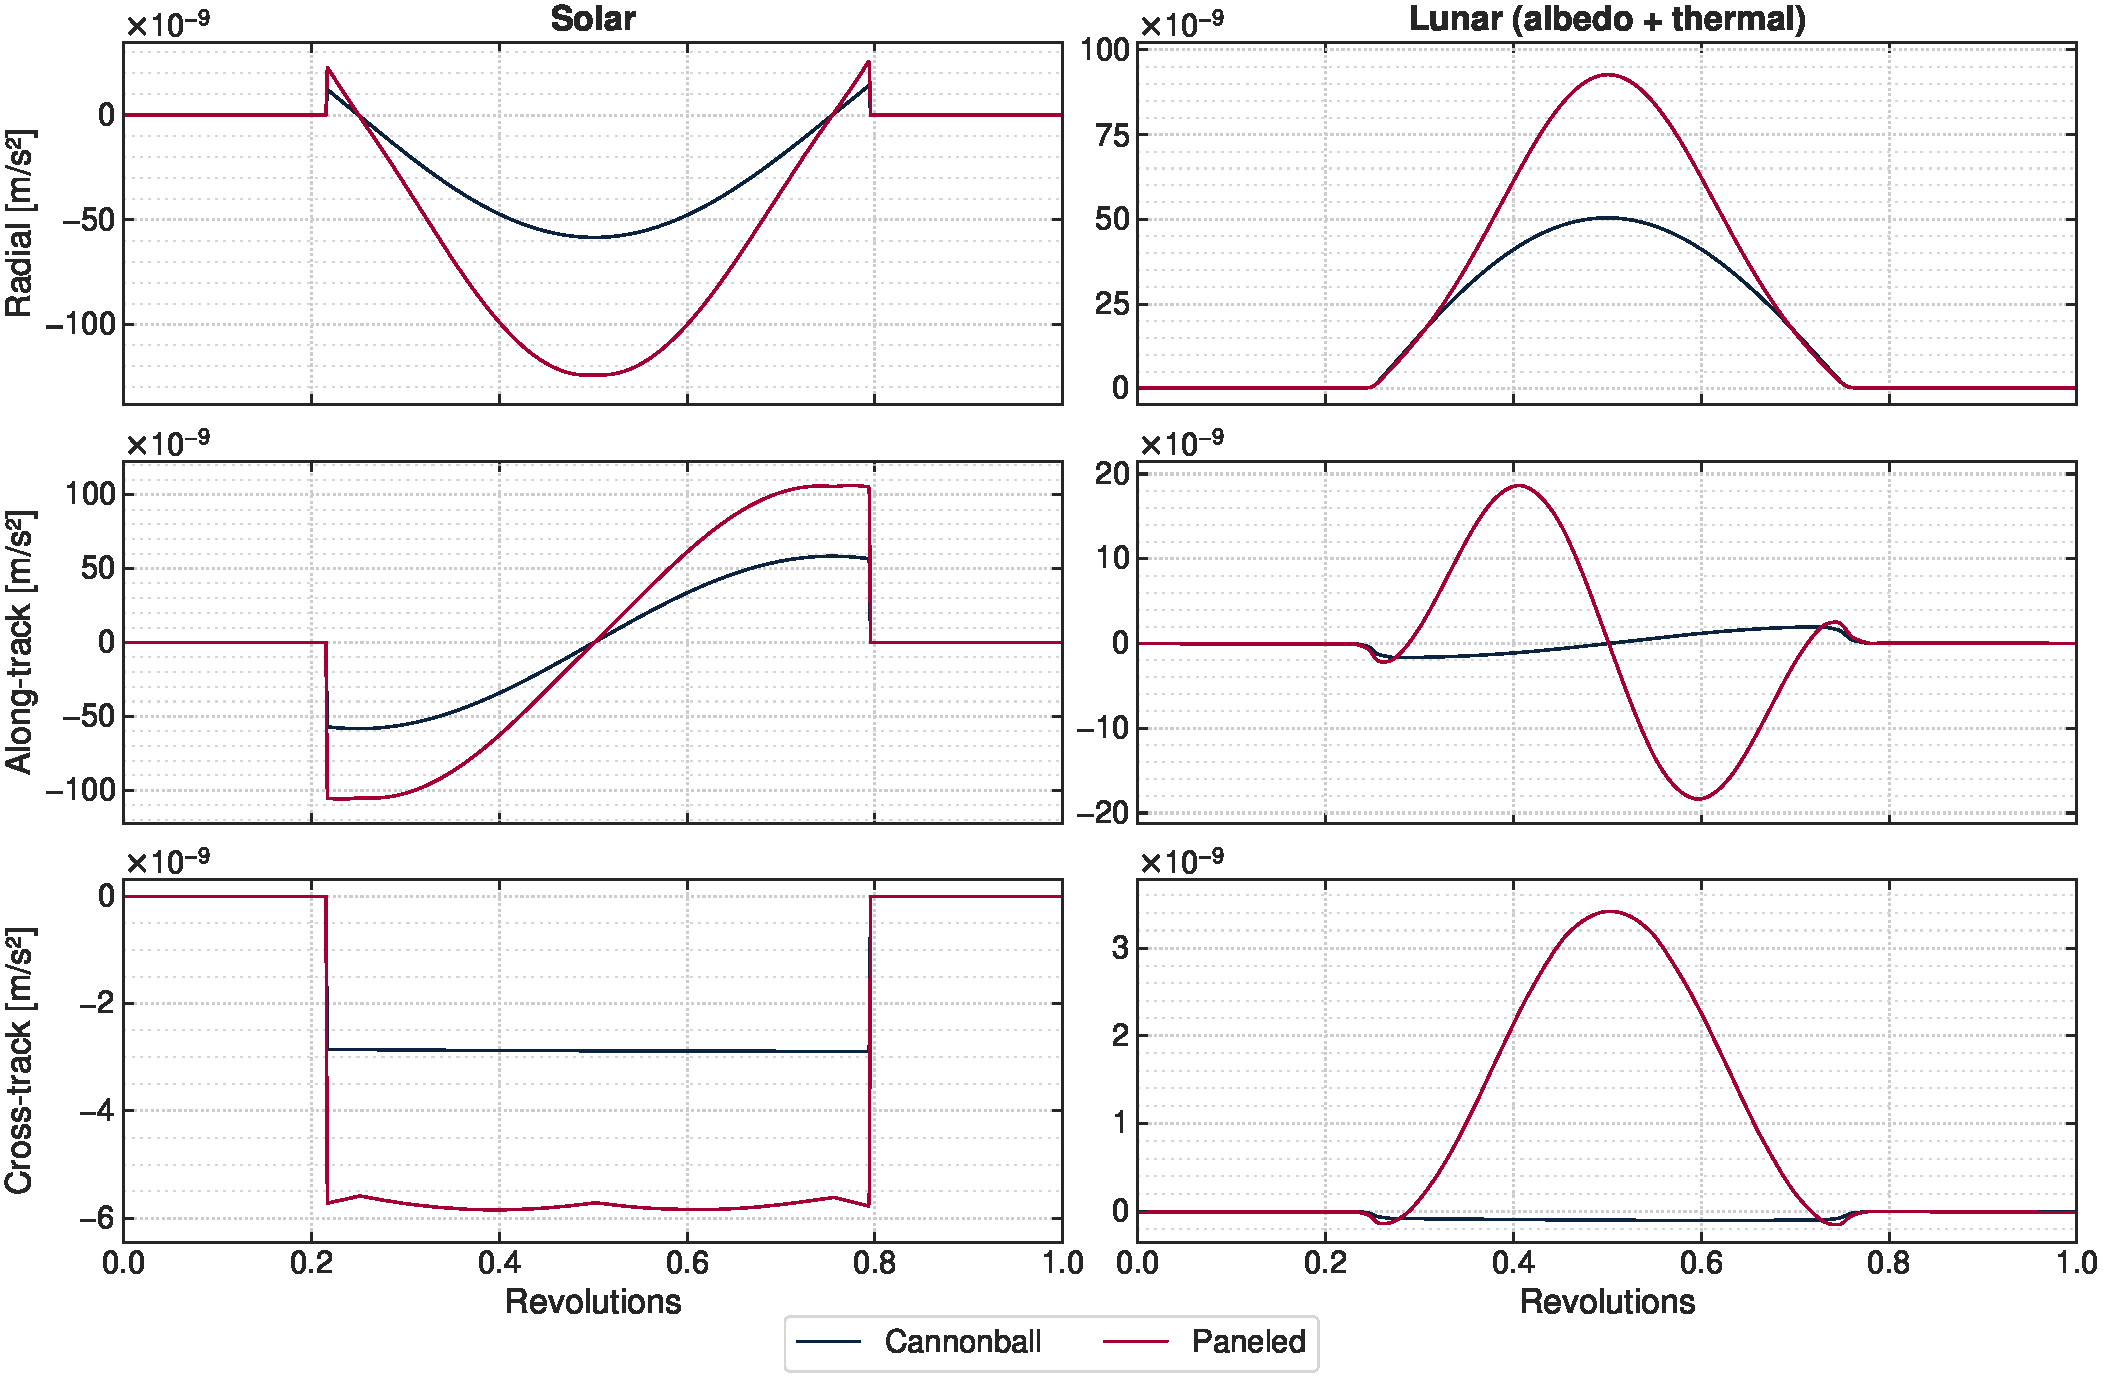
\includegraphics[width=\textwidth]{figures/plots/acc_solarvslunar_sep.pdf}
        \subcaption{September}
        \label{fig:acc-solarvslunar-sep}
     \end{subfigure}

    \caption{Accelerations due to solar and lunar radiation over one orbit for a paneled target. The cannonball and paneled target differ both in magnitude and pattern of accelerations. Note the different scales of each subplot.}
    \label{fig:acc-solarvslunar}
\end{figure*}

For the June arc (\cref{fig:acc-solarvslunar-jun}), the spacecraft is in permanent sunlight and orbit plane normal points towards the sun because $\beta \approx \qty{90}{\degree}$. This leads to extremely large, constant cross-track solar accelerations. The paneled model also has along-track solar accelerations due to the solar array as explained in \cref{subsec:inst-rerad}. Interestingly, the radial solar accelerations show the same phase shift between the cannonball and paneled target as observed without instantaneous reradiation (\cref{subsec:inst-rerad}). This suggests that symmetry is the cause of the phase shift. The magnitude of the total solar acceleration does not change much throughout the year since it is only dependent on the Moon--Sun distance, which is relatively constant at \qty{1}{\astronomicalunit} (see \cref{tab:orbit-geometry}).

The lunar accelerations during the June arc are generally small (less than \qty{2}{\percent} of solar) because \gls{LRO} never passes over well-illuminated regions; half of the lunar source panels that are visible by \gls{LRO} are on the nightside and therefore rarely contribute. The variations in lunar radiation pressure are mainly caused by the fact that $\beta$ is not exactly \qty{90}{\degree} and \gls{LRO}'s angle to the subsolar point therefore varies by \qty{2}{\degree}. Secular variations in lunar accelerations (not shown) are due to the evolution of eccentricity over the 2.5 days caused by the non-uniform lunar gravity field~\cite{Tooley2010}. The eccentricity ranges from 0.005 to 0.008, which leads to periselene altitudes between \qty{37}{\km} and \qty{41}{\km}. Changes in ecentricity lead to larger amplitudes but no mean shift. Periodic variations in altitude due to the eccentricity itself have a minimal effect since higher altitudes mean larger distances but also a larger visible area of the lunar surface, which roughly cancels.

For the September arc (\cref{fig:acc-solarvslunar-sep}), the Sun is occulted for \qty{42}{\percent} of the orbit since $\beta \approx \qty{0}{\degree}$. The effect of these occultations is clearly visible in solar and lunar radiation, both of which vanish on the nightside. The accelerations are mostly in the radial and along-track directions. This is most clearly explained with the solar accelerations. At 0.2, \gls{LRO} crosses the terminator above the pole and is moving straight towards the Sun; the along-track component is maximal and negative since the Sun opposes the spacecraft's motion. Continuing the orbit, \gls{LRO} passes above the subsolar point at 0.5, leading to a maximal and negative radial component while the along-track component has vanished. Further towards the other pole, \gls{LRO} passes into the night at 0.8, where the along-track component accelerates the spacecraft into the direction of motion. During the whole time, the cross-track component is slightly negative because $\beta$ is slightly negative but not zero. If $\beta$ were slightly positive, the cross-track component would be similar but with the sign flipped. The same holds for changes in orbital elements, particularly the inclination and longitude of the ascending node. In addition to periodic changes, there is a secular change in solar accelerations (not shown) since the already slightly negative $\beta$ continues to decrease: over the 2.5 day arc, the mean of the along-track and cross-track components increase twofold and threefold, respectively. This trend continues until the cross-track component dominates for high $\beta$, as seen for the June arc.

The lunar accelerations during the September arc are much larger than during the June arc because \gls{LRO} passes right over the subsolar point, which reflects much sunlight and has high thermal emissions. Indeed, the lunar irradiance (up to \qty{1831}{\irr}) is larger than the solar irradiance (up to \qty{1362}{\irr}) above the subsolar point. Still, the lunar acceleration magnitude is \qty{14}{\percent} smaller than the solar acceleration magnitude since lunar panels are distributed azimuthally around the nadir and thus partially cancel while all solar rays are parallel. Another feature of lunar accelerations is the sign opposite to solar accelerations: when passing over the subsolar point, the radial components of solar and lunar accelerations roughly cancel. A similar effect can be seen in the along-track and cross-track components for a paneled target, although the lunar radiation needs some time to build up. The along-track component peaks at a subsolar angle of \qty{33}{\degree}, the cross-track component above the subsolar point. The cross-track component increases secularly over the 2.5 day arc, similarly to solar radiation.

Comparing the accelerations of cannonball and paneled targets for both arcs, it is clear that a single $C_r$ cannot capture the complex and changing spacecraft geometry. While the solar accelerations for the September arc are just off by about a constant factor, this is not the case for the June arc or any of the lunar accelerations. In fact, the sign may even be different, particularly for lunar along-track and cross-track accelerations in September. This is likely caused by the solar array tracking the Sun. On smaller scales, the effect of target panels of different size and reflective properties becoming visible as \gls{LRO} revolves around the Moon can be seen in the shape of the solar cross-track accelerations of the September arc.

All accelerations are inversely proportional to the spacecraft mass. While we chose the end-of-mission mass for all simulations, the begin-of-mission mass is \qty{17}{\percent} higher and all accelerations are thus \qty{17}{\percent} lower (see \cref{subsec:lro-target}). This only changes magnitudes, not patterns.





\subsubsection{Lunar albedo and thermal radiation}
In the previous subsection, lunar radiation was considered as the sum of albedo and thermal radiation. In this subsection, we look at the separate contributions and the differences between albedo distributions. The accelerations on a paneled targetare shown in \cref{fig:acc-albedovsthermal}.

\begin{figure*}[t]
    \centering
    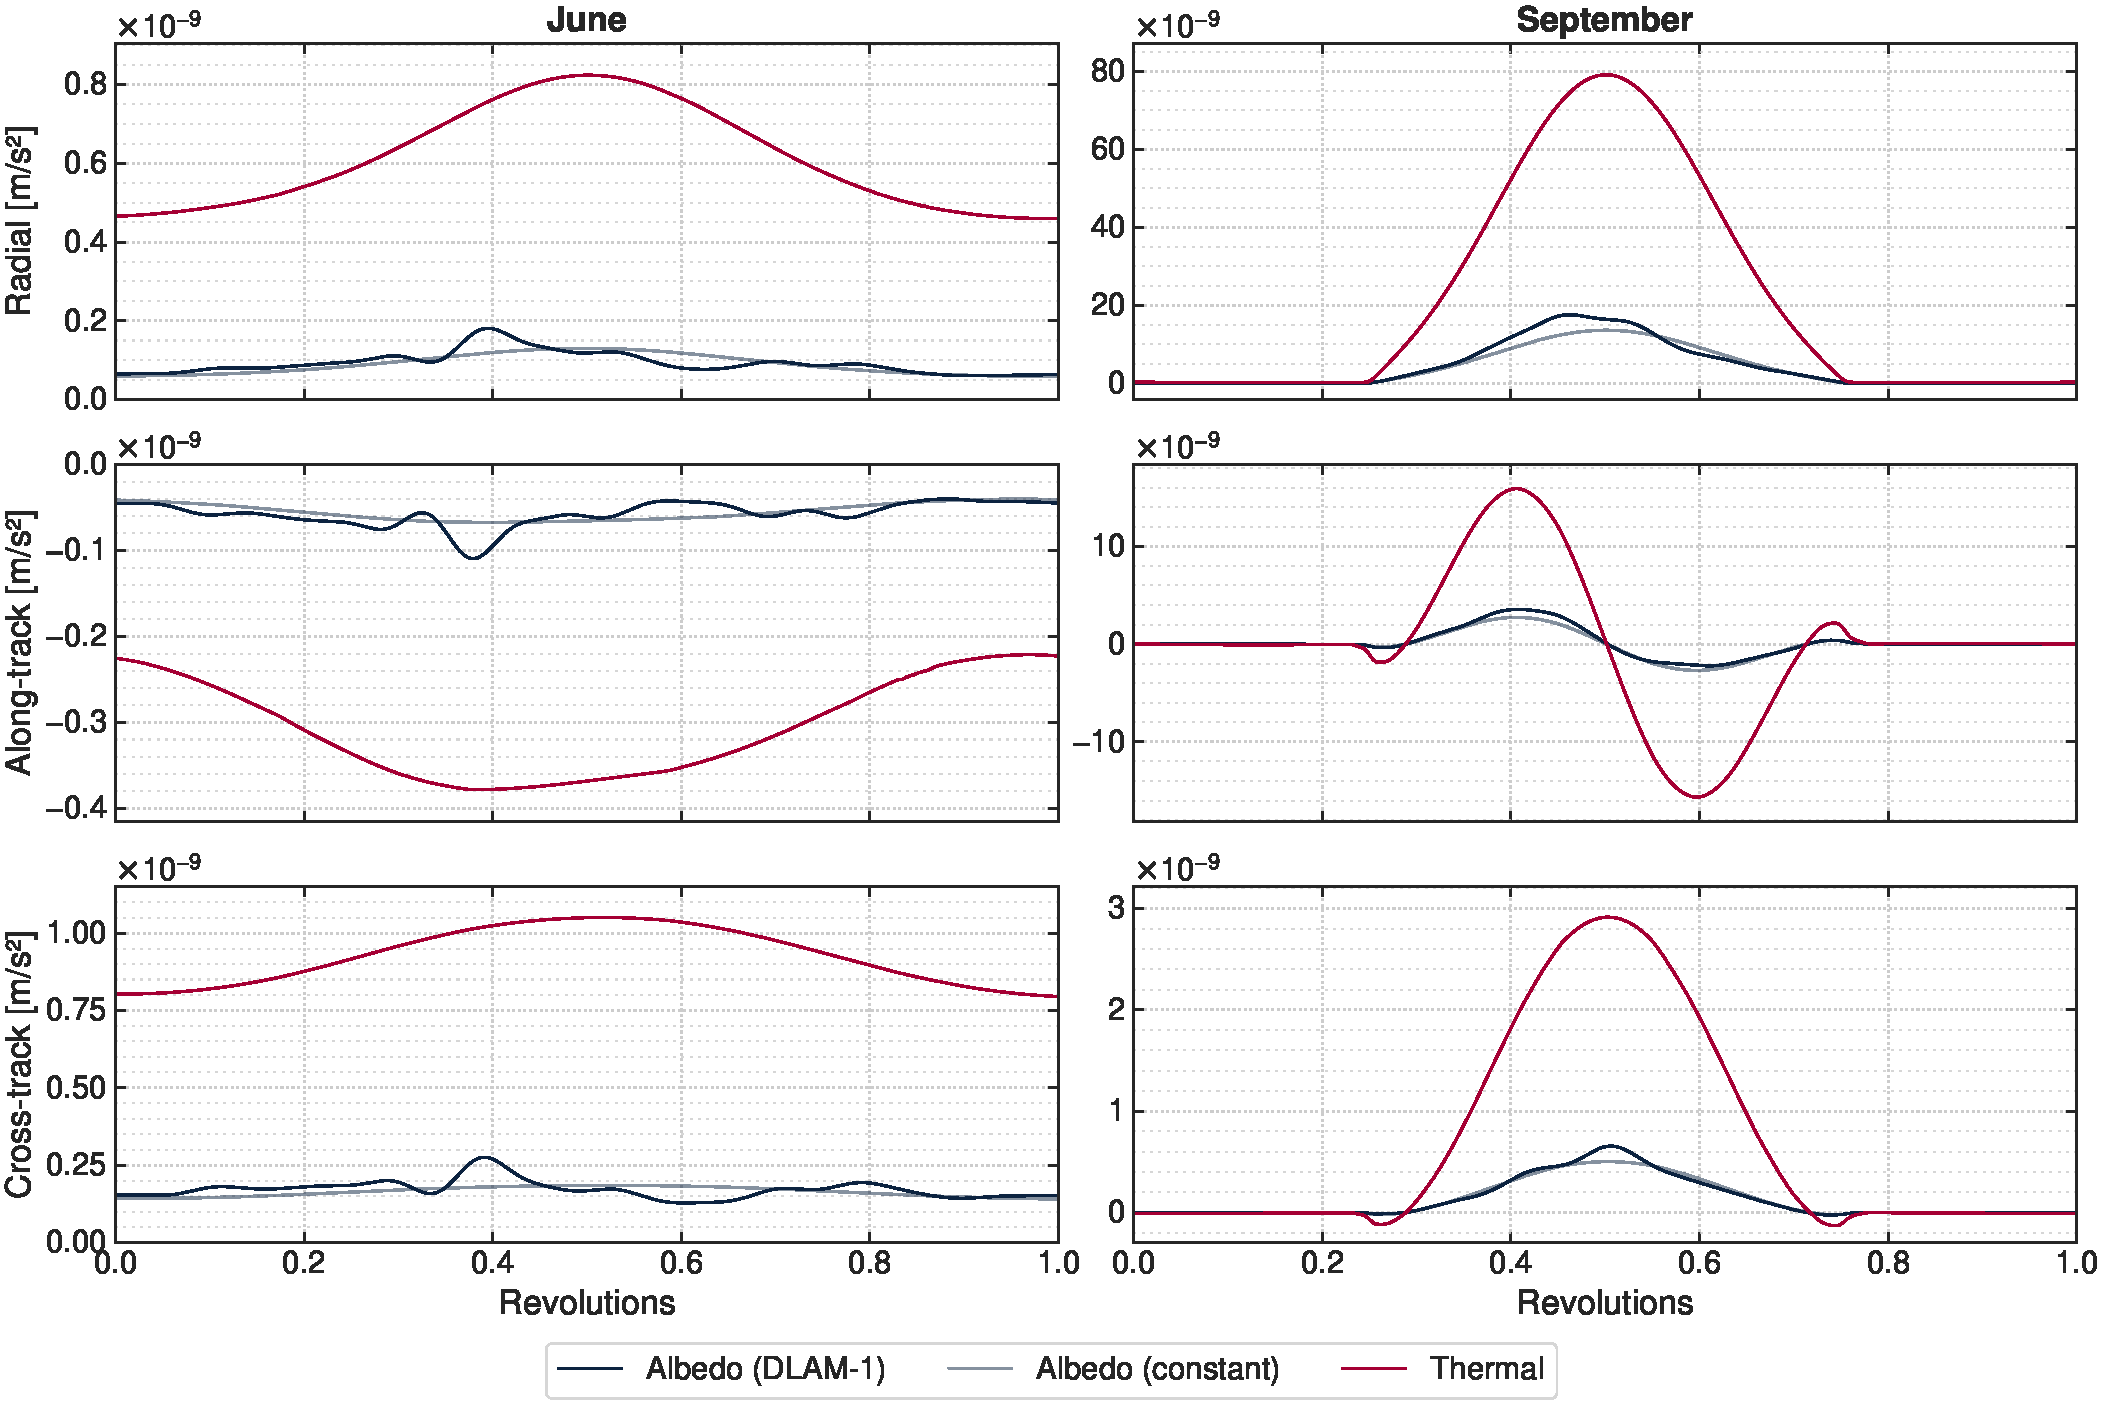
\includegraphics[width=\textwidth]{figures/plots/acc_albedovsthermal.pdf}

    \caption{Accelerations due to lunar thermal and albedo radiation on a paneled target. Thermal radiation dominates at all times and the difference between constant and \gls{DLAM1} albedo is small. Note the different scales of each subplot.}
    \label{fig:acc-albedovsthermal}
\end{figure*}

For both arcs and all components, thermal radiation is far larger than albedo radiation (up to sixfold). This is even though the albedo is likely overestimated by \qty{25}{\percent} as described in \cref{subsec:lunar-albedo}.


\begin{figure}[t]
    \centering
    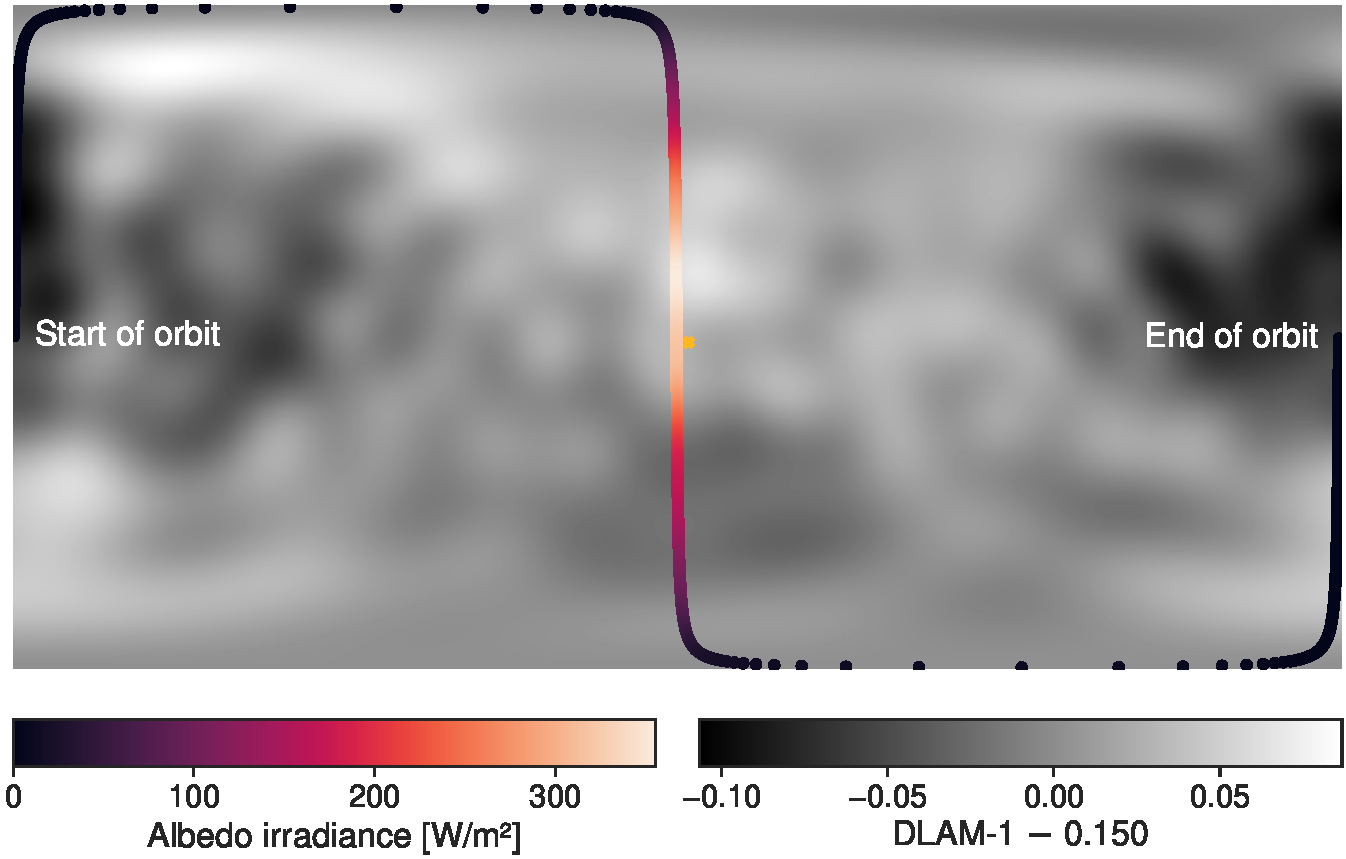
\includegraphics[width=\linewidth]{figures/plots/groundtrack.pdf}
    \caption{Ground track for September arc.}
    \label{fig:groundtrack}
\end{figure}


beta angle slightly less than 90 degrees leads to sinusoidal acceleration in June arc

angle-based thermal behaves quite similar to albedo, but does not vanish in eclipse
both affected by occultation


lunar RP dominated by thermal such that variations from DLAM1 are too small to have effect

max difference \qty{5e-9}{\acc}, find location on map via lat/lon -> corresponds to large deviation from mean in dlam1
maximum occurs before subsolar point
give rms difference








\subsection{Change in final position}

no knowledge of true RP accelerations
therefore, compare to baseline

Also use~\cite{Borderies1990} as reference for plots and discussion, especially about relation of acc and change in elements

Thermal in the range of a few meters ~\cite{Mazarico2011}

Thermal lunar radiation may cause an offset of 1-2 meters over an arclength of 2.5 days~\cite{Bauer2016}

not having moon leads to larger decrease because the sun radial component is not cancelled

prediction september: change in arg peri because solar along-track acts fully above poles without being cancelled by lunar rad

for september: sign of change of inclination and lon asc node depends on sign of beta


\subsection{Change in orbital element}

compare wih Gauss perturbing equations (analytical solution to change of osculating elements based on accelerations), e.g. ~\cite[Sec.~3.2]{Lucchesi2006}

Keplerian state wrt ECLIPJ2000, not Moon frame!!




\subsection{Performance}
no special setup like cpu pinning or disabled hyperthreading for benchmarking
only on one setup
Performance may vary in other situations~\cite{Mytkowicz2009}
still, a good indication
also mention minimum

albedo model can increase computational demand by several hundred pct \cite{Nicholson2010}

